\documentclass[a4j,10pt]{jsarticle}
\usepackage{layout,url,resume}
\usepackage[dvipdfmx]{graphicx}
\pagestyle{empty}

\begin{document}
%\layout

\title{スマートフォンのブラウザで視聴中のWebページ・動画の視聴位置を保存・復旧するしおりアプリ}

% 和文著者名
\author{
    Arch B3 新真虎(masatora) \thanks{慶應義塾大学環境情報学部}
    \and
    Adviser: 松谷健史(macchan) \thanks{慶應義塾大学大学院 政策・メディアメディア研究科特任講師}
}

% 和文概要
\begin{abstract}
ホセ・アブレイユ
\end{abstract}

\maketitle
\thispagestyle{empty}

\section{背景}
スマートフォンでネットサーフィンをしているとき、
読んでいる途中のページや動画を保存したいというニーズがある[]。
そうしたニーズに対応するブックマークアプリはすでに存在する[]。

しかし、既存のブックマークアプリには以下の問題がある。
\begin{enumerate}
\item 保存したWebページのスクロール位置がわからなくなる
\item 保存した動画の再生位置(何分何秒まで見ていた・何分何秒が面白かった)がわからなくなる
\end{enumerate}

その結果、Webページや動画の視聴を再開したり、誰かに共有するたびに、
どこまで読んでいたか・見ていたかを探す時間が無駄になってしまう。

%---------------------------------------------

\section{目的}
上記の問題を解決するため、スマートフォンで見ているWebページや動画をどこまで読んでいたか・
どこまで見ていたかという情報とともに保存し、復旧できるようにすることを目指す。

\section{アプローチ}
Webページおよび動画のスクロール位置や再生位置を保存・復旧することのできる
iOSアプリケーションを開発する。

\section{環境}
タランチュラ

\section{実装}
う

\section{評価}
評価では、開発したアプリケーションが以下の2つの機能を実現できていることを確認する。
\begin{enumerate}
\item 保存したWebページのスクロール位置が復旧できること
\item 保存した動画の再生位置が復旧できること
\end{enumerate}

\section{結果}
\subsection{実現できたこと}

\subsection{実現できていないこと}

\section{記法参考}
\subsection{hoge}
小見出し付きの文章.

\begin{enumerate}
\item 番号付き箇条書き 
\item 番号付き箇条書き
\end{enumerate}

\begin{itemize}
\item 箇条書き
\item 箇条書き
\end{itemize}

\subsection{hoge}
画像を図\ref{sample}に示す。

\begin{figure}[htbp]
    \begin{center}
        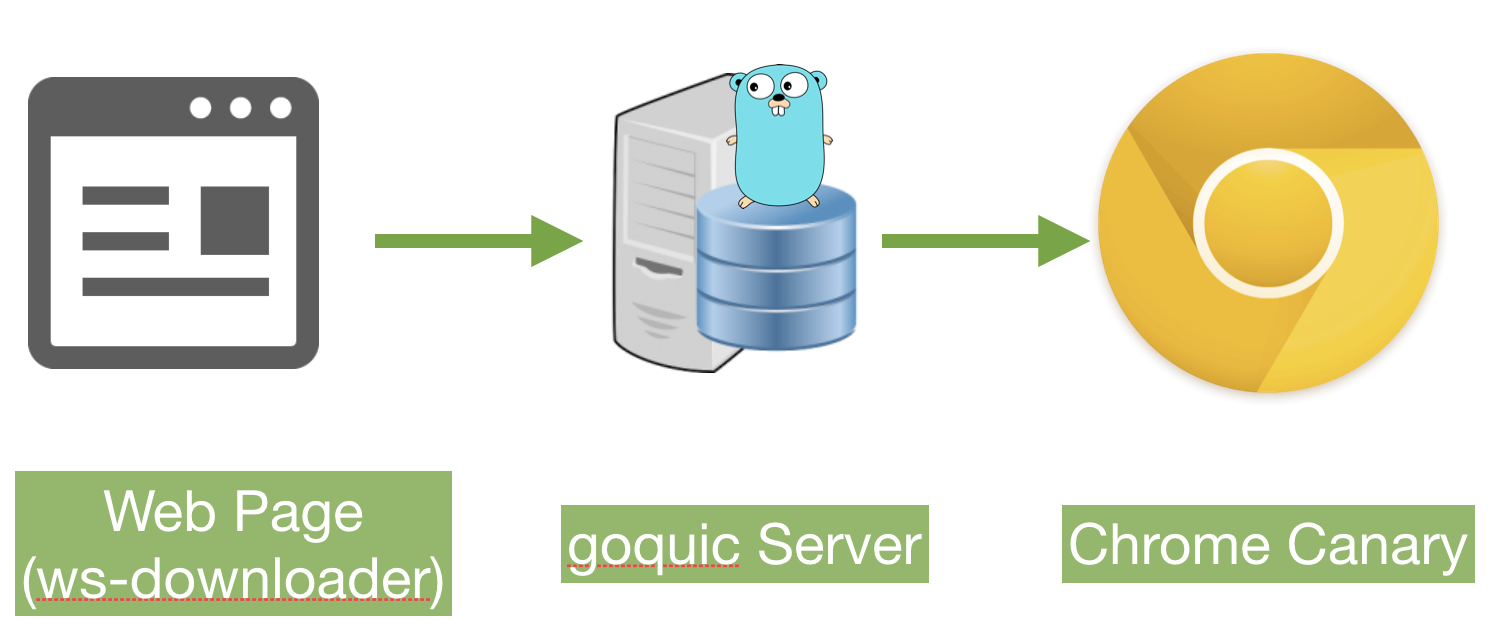
\includegraphics[width=6cm]{figure1.png}
        \caption{画像の例}
        \label{sample}
    \end{center}
\end{figure}


\bibliography{resume}
\bibliographystyle{junsrt}

\end{document}
% end of file
